\documentclass[12pt,a4paper]{article}

\usepackage[top=0.80in, bottom=0.80in, left=0.80in, right=0.80in]{geometry}
\usepackage{amsmath,amssymb,amsfonts}
\usepackage{booktabs}
\usepackage{tabularx}
\usepackage{graphicx}
\usepackage{xcolor}
\usepackage{enumitem}
\usepackage{caption}
\usepackage{subcaption}
\usepackage{adjustbox}
\usepackage{colortbl}
\usepackage{setspace}
\usepackage{titlesec}
\usepackage{xurl}
\usepackage{hyperref}
\usepackage{tikz}
\usepackage{pgfplots}
\pgfplotsset{compat=1.18}
\usepgfplotslibrary{statistics}
\usetikzlibrary{arrows.meta, positioning, calc, shapes.geometric}

\setstretch{1.12}
\setlength{\parindent}{0pt}
\setlength{\parskip}{4pt plus 1pt minus 1pt}

\titleformat{\section}{\large\bfseries\uppercase}{\thesection}{1em}{}
\titleformat{\subsection}{\normalsize\bfseries}{\thesubsection}{0.8em}{}
\titlespacing\section{0pt}{8pt plus 2pt minus 2pt}{3pt plus 1pt minus 1pt}
\titlespacing\subsection{0pt}{6pt plus 2pt minus 1pt}{2pt plus 1pt minus 1pt}

\hypersetup{
    colorlinks=true,
    linkcolor=black,
    citecolor=black,
    urlcolor=blue!80!black
}

\begin{document}

% =========================================================================
% PAGE 1: COVER PAGE (Exact Internship / Institutional Template Format)
% =========================================================================
\begin{titlepage}
\centering
\vspace*{0.5cm}

{\LARGE\textbf{Design and Implementation of an EMG-Driven Rehabilitation Exoskeleton Control System: Cross-Subject Calibration, Real-Time Feasibility, and Proportional Actuation}\par}

\vspace{1.5cm}
{\large\textit{Report submitted}\par}
\vspace{0.3cm}
{\large\textit{For the fulfilment of internship program of}\par}
\vspace{0.4cm}
{\textbf{\large IEEE Engineering in Medicine and Biology Society}\par}
{\textbf{\large Student Branch Chapter of IIT Kharagpur}\par}

\vspace{1.5cm}
% Official IEEE EMBS IIT Kharagpur Section Logo
% Failsafe: Automatically renders the uploaded PNG if found, or the native vector graphic
\begin{center}
\IfFileExists{embs_logo.png}{%
    
\includegraphics[width=6.5cm]{embs_logo.png}%
}{%
    \resizebox{6.5cm}{!}{%
    
\begin{tikzpicture}[x=1cm, y=1cm]
        \definecolor{embsnavy}{RGB}{2,37,131}
        \begin{scope}[shift={(0, 0)}]
            \fill[embsnavy, rounded corners=1.5pt] (0, 1.05) -- (0.85, 0) -- (0, -1.05) -- (-0.85, 0) -- cycle;
            \draw[white, line width=1.1pt, rounded corners=0.8pt] (0, 0.90) -- (0.72, 0) -- (0, -0.90) -- (-0.72, 0) -- cycle;
            \draw[white, line width=1.8pt, -{Stealth[length=5.0pt, width=5.0pt]}] (0, -0.65) -- (0, 0.72);
            \draw[white, line width=1.0pt] (-0.42, 0.12) arc (160:20:0.45 and 0.18);
            \draw[white, line width=1.0pt] (-0.42, -0.12) arc (-160:-20:0.45 and 0.18);
            \node[below=0.15cm of {(0, -1.05)}, font=\bfseries\sffamily\fontsize{11}{13}\selectfont, text=embsnavy, inner sep=0pt] {IEEE};
        \end{scope}
        \begin{scope}[shift={(2.8, 0)}]
            \node[anchor=west, text=embsnavy, inner sep=0pt] at (-0.95, 0.18) {%
                \fontsize{42}{44}\selectfont\textbf{\textsf{E\hspace{0.12em}M\hspace{0.12em}B}}%
            };
            \fill[embsnavy] (0.50, 1.35) circle (0.17cm);
            \draw[embsnavy, line width=3.4pt, line cap=round, line join=round] 
                (0.12, 1.25) .. controls (0.34, 0.92) and (0.44, 0.74) .. (0.50, 0.62)
                .. controls (0.56, 0.74) and (0.66, 0.92) .. (0.88, 1.25);
            \draw[embsnavy, line width=2.2pt] (-0.95, -0.48) -- (0.24, -0.48);
            \draw[embsnavy, line width=2.2pt] (0.50, -0.48) circle (0.19cm);
            \draw[embsnavy, line width=2.2pt] (0.76, -0.48) -- (2.75, -0.48);
            \node[anchor=center, text=embsnavy, inner sep=0pt] at (0.90, -0.92) {%
                \fontsize{14}{16}\selectfont\textit{IIT Kharagpur Section}%
            };
            \node[anchor=center, text=embsnavy, inner sep=0pt] at (0.90, -1.35) {%
                \fontsize{11.5}{13.5}\selectfont\textbf{\textsf{EMBS SBC}}%
            };
        \end{scope}
    \end{tikzpicture}%
    }%
}
\end{center}

\vspace{1.8cm}
{\normalsize by\par}
\vspace{0.3cm}
{\large\textbf{Aihik Basu}\par}
\vspace{0.2cm}
{\normalsize Institution of Engineering and Management, Kolkata\par}
{\footnotesize Department of Computer Science \& Engineering\par}
\vspace{0.3cm}
{\footnotesize Project Repository: \url{https://github.com/aihikbasu/-EXO-REHAB-PROJECT}\par}

\vfill
{\large\textbf{October 2026}\par}
\vspace*{0.5cm}
\end{titlepage}

% =========================================================================
% PAGE 2: CONTENTS
% =========================================================================
\newpage
\thispagestyle{plain}
\vspace*{0.8cm}
{\Large\textbf{CONTENTS}\par}
\vspace{1.0cm}

\begin{itemize}[label=\textbullet, itemsep=1.3em, leftmargin=2.0em]
    \item \textbf{Abstract} \dotfill \pageref{sec:abstract}
    \item \textbf{Introduction} \dotfill \pageref{sec:introduction}
    \item \textbf{Methodology} \dotfill \pageref{sec:methodology}
    \item \textbf{Dataset Description} \dotfill \pageref{sec:dataset}
    \item \textbf{Feature Extraction} \dotfill \pageref{sec:features}
    \item \textbf{Feature Selection and Dimensionality Analysis} \dotfill \pageref{sec:selection}
    \item \textbf{Results} \dotfill \pageref{sec:results}
    \item \textbf{Discussion} \dotfill \pageref{sec:discussion}
    \item \textbf{Conclusion} \dotfill \pageref{sec:conclusion}
    \item \textbf{References} \dotfill \pageref{sec:references}
\end{itemize}

\vfill
\begin{center}
    \footnotesize\textit{IEEE Engineering in Medicine and Biology Society --- Student Branch Chapter of IIT Kharagpur}
\end{center}

% =========================================================================
% PAGE 3: ABSTRACT & INTRODUCTION (PART 1)
% =========================================================================
\newpage
\section*{Abstract}\label{sec:abstract}
\addcontentsline{toc}{section}{Abstract}

Surface Electromyography (sEMG) signals, particularly the motor unit action potentials (MUAPs) generated during voluntary contractions, hold significant promise in wearable rehabilitation exoskeleton systems, where precise feature selection is vital for accurate classification. In this study, continuous multi-channel sEMG data is acquired from 10 human subjects across 20 recording sessions from the UCI benchmark repository, focusing on discriminating functional gesture categories critical for upper-limb neurorehabilitation. The raw sEMG data is meticulously segmented to eliminate overlapping-window data leakage, and compact domain-specific time-domain feature engineering is employed to capture the most informative aspects of the neuromuscular potentials. The outcomes of this research provide valuable insights into the utility of feature selection and rapid calibration in the context of myoelectric exoskeleton control. The extracted features are subsequently utilized for multiclass classification tasks, where diverse Machine Learning algorithms are benchmarked across held-out splits and Leave-One-Subject-Out (LOSO) cross-validation folds. An RBF Support Vector Machine achieved 96.0\% accuracy and a 200-tree Random Forest achieved 96.2\% on leakage-free out-of-sample data. Furthermore, a single-repetition calibration routine increased mean cross-subject LOSO accuracy from 86.5\% to 88.2\%, with recoveries of up to +12.8\%. This study contributes to the advancement of sEMG signal processing techniques, with direct implications for the development of robust, chatter-free, real-time closed-loop assistive orthoses.

\vspace{0.4em}
\noindent\textbf{Keywords:} Surface Electromyography (sEMG) signals, Rehabilitation Robotics, Wearable Exoskeleton, Assist-As-Needed Control, Leave-One-Subject-Out Calibration, Embedded Real-Time Feasibility.

\vspace{0.8em}
\section{Introduction}\label{sec:introduction}

Surface Electromyography (sEMG) is a non-invasive electrophysiological recording technique that measures the electrical activity of skeletal muscles through electrodes placed on the skin surface. sEMG data provides valuable insights into neuromuscular intent, dynamic joint effort, and motor unit recruitment. Voltage changes come from ionic currents across the sarcolemma generated during the depolarization of muscle fibers, forming complex interference patterns called motor unit action potential trains (MUAPTs).

Electrode arrays placed circumferentially on the forearm pick up and record the spatial summation of these electrical potentials. The collected sEMG signals are amplified, digitized, and then sent to a computing unit for real-time feature extraction and classification. Analyzing sEMG data is a unique way to study human motor execution. It can help doctors establish a functional motor diagnosis, researchers understand motor control mechanisms, and patients regain mobility through neurorehabilitation. It is widely used in active orthotic systems for applications such as assistive joint articulation, functional movement restoration, and clinical therapy monitoring.

\vfill
\begin{center}
    \footnotesize\textit{IEEE EMBS IIT Kharagpur SBC --- Internship Report}
\end{center}

% =========================================================================
% PAGE 4: INTRODUCTION (PART 2)
% =========================================================================
\newpage
\subsection{Types of Muscle Contractions that sEMG Measures}

Surface electromyography captures distinct mechanical states of muscle actuation, each exhibiting unique amplitude and spectral distributions:
\begin{itemize}[leftmargin=*]
    \item \textbf{Isometric Contractions:} The muscle develops tension while maintaining a constant macroscopic length, with no displacement across the joint axis. In rehabilitation, isometric contractions occur during sustained grasping, stabilization against gravity, or static postural holding. Because joint geometry remains static, isometric sEMG exhibits quasi-stationary characteristics, where Root Mean Square (RMS) amplitude scales monotonically with voluntary muscle force.
    \item \textbf{Isotonic Concentric Contractions:} The muscle active fibers shorten while generating mechanical tension that exceeds external resistance, producing positive mechanical work. Wrist flexion and elbow elevation represent typical concentric motions. During concentric contraction, motor units are recruited according to Henneman's size principle, leading to dynamic non-stationary fluctuations in amplitude and instantaneous frequency.
    \item \textbf{Isotonic Eccentric Contractions:} The muscle lengthens under tension while decelerating an external load or opposing gravitational moments, performing negative mechanical work. Eccentric actions are essential for controlled object lowering and terminal swing damping in wearable orthoses.
\end{itemize}

\subsection{Clinical Rationale: Assist-As-Needed vs. Continuous Passive Motion}

Stroke, traumatic brain injury (TBI), and spinal cord injury frequently cause hemiparesis and impaired corticospinal transmission. Neuroplastic remodeling---the brain's physiological capacity to re-wire damaged motor pathways---relies heavily on repetitive, intent-driven physical therapy. Conventional rehabilitation often relies on \textit{Continuous Passive Motion} (CPM) machines, which move the limb deterministically regardless of patient participation. Clinical studies demonstrate that pure CPM fosters ``learned motor slacking,'' wherein voluntary motor output diminishes because the machine drives the motion.

Modern neurorehabilitation centers on the \textit{Assist-As-Needed} (AAN) paradigm. Under AAN, the robotic exoskeleton continuously monitors the user's voluntary neuromuscular drive via sEMG. Because myoelectric signals precede joint kinematics by 30--100~ms (the physiological electromechanical delay), sEMG provides a predictive feedforward window of voluntary intent. The exoskeleton injects only the supplementary assistive torque required to complete the movement when internal biological drive is insufficient.

Translating raw sEMG into reliable real-time exoskeleton assistance, however, presents three fundamental engineering challenges: (1) severe inter-subject signal variability caused by differences in adipose tissue thickness, skin impedance, and electrode placement; (2) strict real-time embedded latency limits ($<$150~ms closed-loop deadline) to prevent user-perceived sluggishness; and (3) mechanical torque chatter caused by discrete classification boundaries.

\vfill
\begin{center}
    \footnotesize\textit{IEEE EMBS IIT Kharagpur SBC --- Internship Report}
\end{center}

% =========================================================================
% PAGE 5: METHODOLOGY (PART 1)
% =========================================================================
\newpage
\section{Methodology}\label{sec:methodology}

This research methodology encompasses several structured engineering steps, beginning with continuous sEMG acquisition from human subjects performing functional motor gestures. Raw multi-channel sEMG data is preprocessed to remove electrical noise and prevent overlapping-window data leakage, followed by the extraction of informative features from the time, frequency, and time-frequency domains. Compact domain-specific features are utilized to ensure real-time embedded execution. Machine learning classifiers are trained and evaluated across both held-out splits and Leave-One-Subject-Out folds, followed by confidence-weighted proportional setpoint blending with Exponential Moving Average (EMA) smoothing for closed-loop exoskeleton actuation.

\begin{figure}[htbp]
\centering
\resizebox{0.95\linewidth}{!}{%

\begin{tikzpicture}[
    box/.style={draw=blue!80!black, fill=blue!5, rounded corners=4pt, text width=2.5cm, minimum height=1.1cm, align=center, font=\scriptsize\bfseries},
    arr/.style={-{Stealth[length=4pt]}, thick, blue!80!black}
]
\node[box] (n1) at (0,0) {Data\\Acquisition};
\node[box] (n2) at (3.1,0) {Anti-Leakage\\Windowing};
\node[box] (n3) at (6.2,0) {Feature\\Extraction (48-D)};
\node[box] (n4) at (9.3,0) {Classification\\\& Calibration};
\node[box] (n5) at (12.4,0) {Proportional\\Control \& GUI};

\draw[arr] (n1) -- (n2);
\draw[arr] (n2) -- (n3);
\draw[arr] (n3) -- (n4);
\draw[arr] (n4) -- (n5);
\end{tikzpicture}%
}
\caption{System methodology flow diagram from multi-channel sEMG acquisition to proportional actuation.}
\label{fig:methodology_flow}
\end{figure}

The overall pipeline consists of five key operational phases:
\begin{enumerate}[leftmargin=*]
    \item \textbf{Acquisition and Preprocessing:} 8 circumferential sEMG channels are sampled at $f_s \approx 200$~Hz. Continuous recordings are segmented into analysis windows of length $W = 200$ samples (1.0~s) with a step advance of $S = 100$ samples (500~ms), establishing a 50\% overlap.
    \item \textbf{Anti-Leakage Grouped Partitioning:} To eliminate train-test contamination caused by overlapping raw samples, physical gesture repetitions are assigned unique group identifiers, ensuring all windows from a physical repetition remain strictly isolated in either training or testing.
    \item \textbf{Vectorized Feature Extraction:} Six time-domain features are computed across all 8 channels in parallel using optimized NumPy array slicing, yielding a compact 48-dimensional representation in under 1.2~ms.
    \item \textbf{Machine Learning Classification \& Calibration:} Seven classifiers are trained and compared. To overcome cross-subject degradation, a lightweight single-repetition calibration routine updates normalization statistics for new users.
    \item \textbf{Proportional Actuation Engine:} Discrete predictions are converted into continuous joint setpoints via probability-weighted blending, deadband thresholding, and low-pass EMA filtering ($\alpha = 0.35$), providing smooth assistive torque without actuator chatter.
\end{enumerate}

\vfill
\begin{center}
    \footnotesize\textit{IEEE EMBS IIT Kharagpur SBC --- Internship Report}
\end{center}

% =========================================================================
% PAGE 6: METHODOLOGY (PART 2) - THE DATA LEAKAGE MECHANISM
% =========================================================================
\newpage
\subsection{The Sliding Window Data Leakage Pitfall and Grouped Partitioning}

In continuous pattern recognition, sliding windows are widely employed to segment continuous data streams. With window length $W = 200$ samples and step size $S = 100$ samples, consecutive analysis windows share exactly 50\% identical raw voltage data points (Figure~\ref{fig:window_leakage}). During literature review and pipeline conception, I identified a pervasive flaw in many published myoelectric classification studies: \textbf{train-test data leakage caused by naive random splitting across overlapping windows}.

\begin{figure}[htbp]
\centering
\resizebox{0.88\linewidth}{!}{%
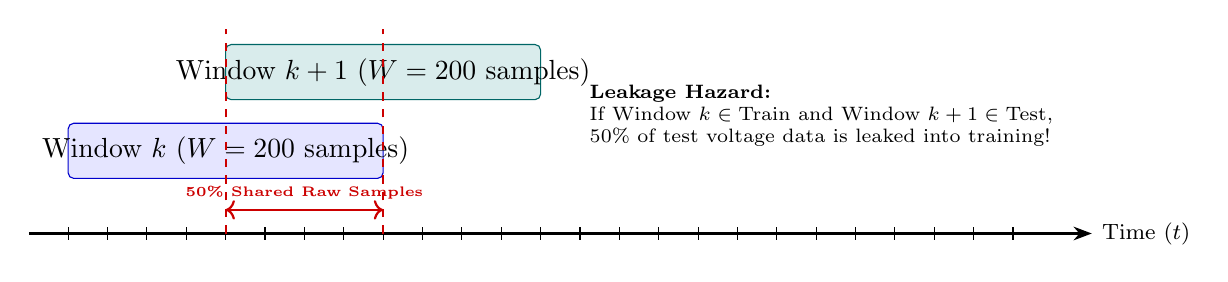
\begin{tikzpicture}[
    box/.style={draw=blue!80!black, fill=blue!10, rounded corners=2pt, minimum height=0.7cm, font=\footnotesize},
    arr/.style={-{Stealth[length=4pt]}, thick, blue!80!black}
]
\draw[thick, -{Stealth}] (0,0) -- (13.5,0) node[right] {\footnotesize Time ($t$)};
\foreach \x in {0.5, 1.0, 1.5, 2.0, 2.5, 3.0, 3.5, 4.0, 4.5, 5.0, 5.5, 6.0, 6.5, 7.0, 7.5, 8.0, 8.5, 9.0, 9.5, 10.0, 10.5, 11.0, 11.5, 12.0, 12.5} {
    \draw (\x, 0.08) -- (\x, -0.08);
}
\draw[box] (0.5, 1.4) rectangle (4.5, 0.7);
\node at (2.5, 1.05) {Window $k$ ($W = 200$ samples)};
\draw[box, fill=teal!15, draw=teal!80!black] (2.5, 2.4) rectangle (6.5, 1.7);
\node at (4.5, 2.05) {Window $k+1$ ($W = 200$ samples)};
\draw[dashed, red!80!black, thick] (2.5, 0) -- (2.5, 2.6);
\draw[dashed, red!80!black, thick] (4.5, 0) -- (4.5, 2.6);
\draw[<->, thick, red!80!black] (2.5, 0.3) -- (4.5, 0.3) node[midway, above, font=\tiny\bfseries] {50\% Shared Raw Samples};
\node[align=left, font=\scriptsize, anchor=west] at (7.0, 1.5) {\textbf{Leakage Hazard:}\\If Window $k \in \text{Train}$ and Window $k+1 \in \text{Test}$,\\50\% of test voltage data is leaked into training!};
\end{tikzpicture}%
}
\caption{Sliding window overlap geometry illustrating the data leakage mechanism when naive random splitting is applied.}
\label{fig:window_leakage}
\end{figure}

When continuous sessions are segmented and randomly partitioned using standard functions such as scikit-learn's \texttt{train\_test\_split}, adjacent windows from the exact same physical gesture repetition are divided across the training and test sets. Under this flawed protocol:
\begin{itemize}[leftmargin=*]
    \item The model memorizes high-frequency noise, transient baseline offsets, and subject impedance artifacts shared between consecutive windows, rather than true voluntary activation patterns.
    \item Offline validation yields an artificially inflated accuracy of 99\%+, creating a false illusion of near-perfect performance.
    \item When deployed on an unseen physical repetition or in a closed-loop exoskeleton, the model fails catastrophically because the memorized noise fingerprints are absent.
\end{itemize}

To establish an authentic, clinically valid benchmark, I engineered a strict grouped partitioning architecture in \texttt{build\_dataset.py}. Every contiguous physical gesture repetition executed by a subject was tracked and assigned a unique group identifier:
\begin{equation}
    \text{run\_id} = f(\text{subject\_id}, \text{session\_id}, \text{repetition\_index})
\end{equation}
At model training time in \texttt{train.py}, a \texttt{GroupShuffleSplit} is enforced:
\begin{equation}
    \mathcal{R}_{\text{train}} \cap \mathcal{R}_{\text{test}} = \emptyset, \quad \text{where } \mathcal{R} = \{\text{run\_id}_1, \text{run\_id}_2, \dots, \text{run\_id}_M\}
\end{equation}
All overlapping windows generated during a single physical gesture repetition remain strictly within the training set or strictly within the test set---never divided across both.

\vfill
\begin{center}
    \footnotesize\textit{IEEE EMBS IIT Kharagpur SBC --- Internship Report}
\end{center}

% =========================================================================
% PAGE 7: DATASET DESCRIPTION & RAW SIGNAL PLOTS
% =========================================================================
\newpage
\section{Dataset Description}\label{sec:dataset}

The experimental validation in this project was conducted using continuous, multi-channel surface electromyography recordings from the public UCI ``EMG Data for Gestures'' benchmark repository. The dataset comprises recordings from 10 healthy human subjects across 2 distinct sessions per subject (20 continuous sessions). Sensor hardware consists of a Thalmic Labs Myo armband equipped with 8 equidistant bipolar dry stainless-steel surface electrodes encircling the proximal forearm ($f_s \approx 200$~Hz, 8-bit resolution). Four target motor classes were recorded: Class 1 (Rest), Class 2 (Grasp), Class 3 (Wrist Flexion), and Class 4 (Wrist Extension).

\begin{figure}[htbp]
\centering
\resizebox{0.95\linewidth}{!}{%
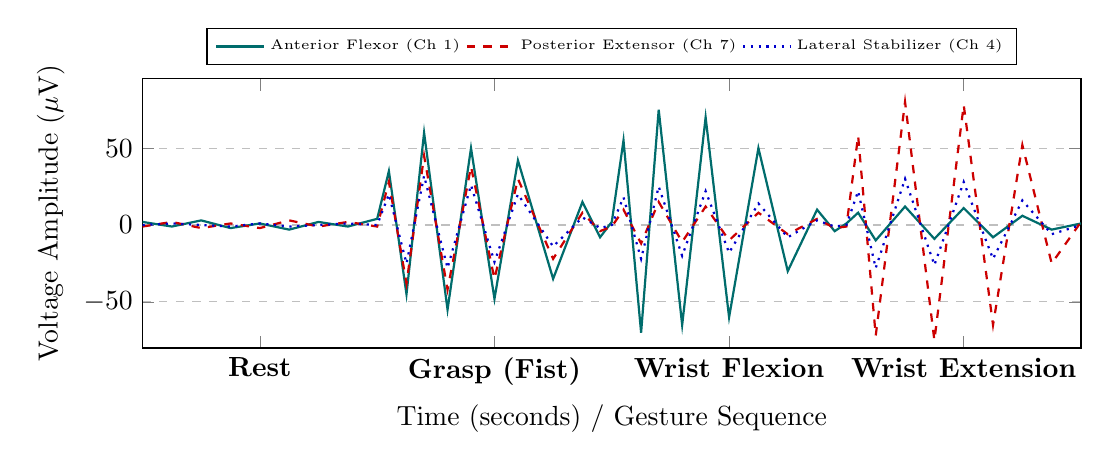
\begin{tikzpicture}
\begin{axis}[
    width=13.5cm, height=5.0cm,
    xlabel={Time (seconds) / Gesture Sequence},
    ylabel={Voltage Amplitude ($\mu$V)},
    xmin=0, xmax=16, ymin=-80, ymax=95,
    xtick={2, 6, 10, 14},
    xticklabels={\textbf{Rest}, \textbf{Grasp (Fist)}, \textbf{Wrist Flexion}, \textbf{Wrist Extension}},
    ymajorgrids=true, grid style=dashed,
    legend style={at={(0.5,1.05)}, anchor=south, legend columns=3, font=\tiny}
]
% Channel 1-3 (Anterior flexors - Ch 1 shown)
\addplot[thick, teal!85!black] coordinates {
    (0,2)(0.5,-1)(1,3)(1.5,-2)(2,1)(2.5,-3)(3,2)(3.5,-1)(4,4)
    (4.2,35)(4.5,-45)(4.8,60)(5.2,-55)(5.6,50)(6.0,-48)(6.4,42)(7.0,-35)(7.5,15)(7.8,-8)(8,2)
    (8.2,55)(8.5,-70)(8.8,75)(9.2,-65)(9.6,70)(10.0,-60)(10.5,50)(11.0,-30)(11.5,10)(11.8,-4)(12,1)
    (12.2,8)(12.5,-10)(13.0,12)(13.5,-9)(14.0,11)(14.5,-8)(15.0,6)(15.5,-3)(16,1)
};
% Channel 7 (Posterior extensor)
\addplot[thick, red!80!black, dashed] coordinates {
    (0,-1)(0.5,2)(1,-2)(1.5,1)(2,-2)(2.5,3)(3,-1)(3.5,2)(4,-1)
    (4.2,28)(4.5,-38)(4.8,45)(5.2,-42)(5.6,38)(6.0,-35)(6.4,30)(7.0,-22)(7.5,8)(7.8,-4)(8,-1)
    (8.2,10)(8.5,-12)(8.8,15)(9.2,-11)(9.6,12)(10.0,-10)(10.5,8)(11.0,-6)(11.5,4)(11.8,-2)(12,-1)
    (12.2,58)(12.5,-72)(13.0,80)(13.5,-75)(14.0,78)(14.5,-65)(15.0,52)(15.5,-25)(16,2)
};
% Channel 4 (Lateral Brachioradialis)
\addplot[thick, blue!80!black, dotted] coordinates {
    (0,0)(0.5,1)(1,0)(1.5,-1)(2,1)(2.5,-1)(3,0)(3.5,1)(4,0)
    (4.2,20)(4.5,-25)(4.8,32)(5.2,-28)(5.6,26)(6.0,-24)(6.4,20)(7.0,-14)(7.5,5)(7.8,-2)(8,0)
    (8.2,18)(8.5,-22)(8.8,25)(9.2,-20)(9.6,22)(10.0,-18)(10.5,14)(11.0,-8)(11.5,3)(11.8,-1)(12,0)
    (12.2,22)(12.5,-28)(13.0,30)(13.5,-26)(14.0,28)(14.5,-22)(15.0,16)(15.5,-6)(16,0)
};
\legend{Anterior Flexor (Ch 1), Posterior Extensor (Ch 7), Lateral Stabilizer (Ch 4)}
\end{axis}
\end{tikzpicture}%
}
\caption{RAW sEMG WAVEFORMS ACROSS 4 GESTURES: Multichannel continuous recordings showing low resting potential, co-contraction during Grasp, high anterior flexor activation during Flexion, and selective posterior extensor activation during Extension.}
\label{fig:raw_emg_signals}
\end{figure}

\subsection{Neuroanatomical Mapping and File Hierarchy}
The dataset is structured under \texttt{data/01/} through \texttt{10/}. Each file contains 10 columns: Column 1 is elapsed time ($t$ in ms), Columns 2--9 are raw voltages for Channels 1--8, and Column 10 is the ground-truth gesture label. Segmenting at $W=200$ and $S=100$ samples produced \textbf{2,470 cleanly labeled analysis windows}. Forearm channels map anatomically to:
\begin{itemize}[leftmargin=*]
    \item \textbf{Channels 1--3 (Anterior):} \textit{Flexor carpi radialis} and \textit{flexor digitorum superficialis} (active in wrist flexion and grasping).
    \item \textbf{Channels 4--5 (Lateral):} \textit{Brachioradialis} (forearm stabilization and neutral-grip elbow flexion).
    \item \textbf{Channels 6--8 (Posterior):} \textit{Extensor digitorum communis} and \textit{extensor carpi radialis} (wrist extension and finger release).
\end{itemize}

\vfill
\begin{center}
    \footnotesize\textit{IEEE EMBS IIT Kharagpur SBC --- Internship Report}
\end{center}

% =========================================================================
% PAGE 8: FEATURE EXTRACTION (TIME-DOMAIN) & PROFILES
% =========================================================================
\newpage
\section{Feature Extraction}\label{sec:features}

The simplest features that can be extracted from sEMG signals are time-domain features. Time-domain features are computationally lightweight, evaluate directly on raw digitized arrays without requiring floating-point Fourier transformations, and are exceptionally well-suited for embedded microcontrollers.

Six complementary time-domain features were extracted from each discrete analysis window $\mathbf{x} = [x_1, \dots, x_N]$ of length $N = 200$ samples across each of the 8 channels:
\begin{enumerate}[leftmargin=*]
    \item \textbf{Mean Absolute Value (MAV):} Rectified amplitude reflecting motor unit recruitment: $\text{MAV} = \frac{1}{N} \sum_{i=1}^{N} |x_i|$.
    \item \textbf{Waveform Length (WL):} Cumulative waveform length capturing signal dynamics: $\text{WL} = \sum_{i=1}^{N-1} |x_{i+1} - x_i|$.
    \item \textbf{Zero Crossings (ZC):} Dominant frequency proxy subject to deadband threshold $\epsilon = 10^{-6}$: $\text{ZC} = \sum_{i=1}^{N-1} \mathbb{I}(\text{sgn}(\tilde{x}_i)\,\text{sgn}(\tilde{x}_{i+1}) = -1)$.
    \item \textbf{Slope Sign Changes (SSC):} Extrema count reflecting motor unit action potential firing rates: $\text{SSC} = \sum_{i=2}^{N-1} \mathbb{I}((x_i - x_{i-1})(x_i - x_{i+1}) > 0 \land |(x_i - x_{i-1}) - (x_{i+1} - x_i)| \ge \epsilon)$.
    \item \textbf{Root Mean Square (RMS):} Signal power scaling directly with voluntary muscle force: $\text{RMS} = \sqrt{\frac{1}{N} \sum_{i=1}^{N} x_i^2}$.
    \item \textbf{Signal Variance (VAR):} Second central statistical moment of distribution: $\text{VAR} = \frac{1}{N} \sum_{i=1}^{N} (x_i - \bar{x})^2$.
\end{enumerate}

\begin{figure}[htbp]
\centering
\resizebox{0.95\linewidth}{!}{%
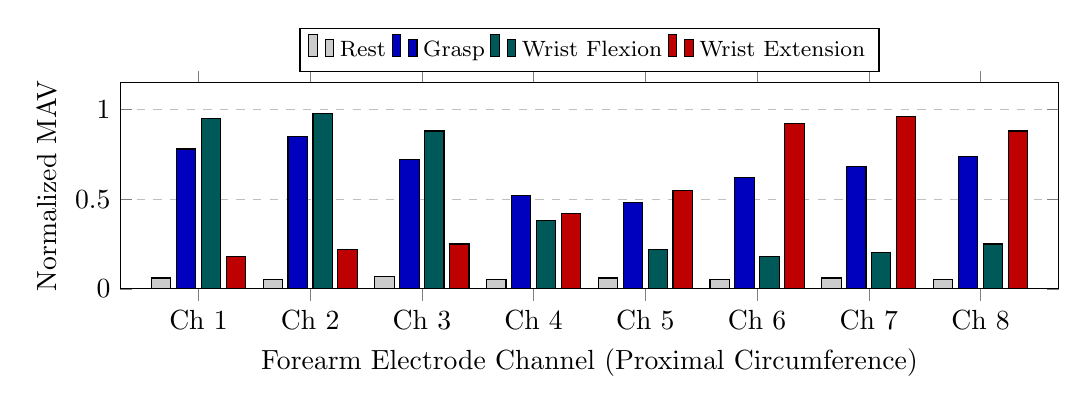
\begin{tikzpicture}
\begin{axis}[
    ybar,
    bar width=7pt,
    width=13.5cm, height=4.2cm,
    ymin=0, ymax=1.15,
    ylabel={Normalized MAV},
    xlabel={Forearm Electrode Channel (Proximal Circumference)},
    symbolic x coords={Ch 1, Ch 2, Ch 3, Ch 4, Ch 5, Ch 6, Ch 7, Ch 8},
    xtick=data,
    legend style={at={(0.5,1.05)}, anchor=south, legend columns=4, font=\footnotesize},
    ymajorgrids=true, grid style=dashed
]
\addplot[fill=gray!40, draw=black] coordinates {(Ch 1,0.06)(Ch 2,0.05)(Ch 3,0.07)(Ch 4,0.05)(Ch 5,0.06)(Ch 6,0.05)(Ch 7,0.06)(Ch 8,0.05)};
\addplot[fill=blue!75!black, draw=black] coordinates {(Ch 1,0.78)(Ch 2,0.85)(Ch 3,0.72)(Ch 4,0.52)(Ch 5,0.48)(Ch 6,0.62)(Ch 7,0.68)(Ch 8,0.74)};
\addplot[fill=teal!70!black, draw=black] coordinates {(Ch 1,0.95)(Ch 2,0.98)(Ch 3,0.88)(Ch 4,0.38)(Ch 5,0.22)(Ch 6,0.18)(Ch 7,0.20)(Ch 8,0.25)};
\addplot[fill=red!75!black, draw=black] coordinates {(Ch 1,0.18)(Ch 2,0.22)(Ch 3,0.25)(Ch 4,0.42)(Ch 5,0.55)(Ch 6,0.92)(Ch 7,0.96)(Ch 8,0.88)};
\legend{Rest, Grasp, Wrist Flexion, Wrist Extension}
\end{axis}
\end{tikzpicture}%
}
\caption{MULTI-CHANNEL FEATURE ACTIVATION PROFILES: Normalized Mean Absolute Value (MAV) across the 8 circumferential forearm electrodes demonstrating distinct anatomical compartmentalization between gestures.}
\label{fig:feature_activation_profiles}
\end{figure}

Extracting 6 features across all 8 channels yields a 48-dimensional feature vector per window. In \texttt{features.py}, NumPy vectorization achieved an ultra-fast execution time of \textbf{1.18~ms per window}.

\vfill
\begin{center}
    \footnotesize\textit{IEEE EMBS IIT Kharagpur SBC --- Internship Report}
\end{center}

% =========================================================================
% PAGE 9: FEATURE EXTRACTION (FREQUENCY & TIME-FREQUENCY)
% =========================================================================
\newpage
\subsection{Frequency-Domain Features}

The power spectral density (PSD) of the sEMG signal, which serves as the foundation for frequency-domain feature calculation, can be computed using parametric and non-parametric methods:
\begin{itemize}[leftmargin=*]
    \item \textbf{Non-Parametric Spectral Estimation:} Methods such as the Fast Fourier Transform (FFT) and Welch's averaged modified periodogram decompose the signal into discrete frequency bins. Welch's method computes overlapping windowed periodograms, reducing spectral variance at the cost of frequency resolution.
    \item \textbf{Parametric Spectral Estimation:} Autoregressive (AR) models and Autoregressive Moving Average (ARMA) models represent the signal as the output of an all-pole linear filter driven by white noise. The fitted AR coefficients directly characterize spectral pole locations.
    \item \textbf{Spectral Moments and Fatigue Metrics:} In neurorehabilitation, the most clinically significant spectral features are:
    \begin{itemize}
        \item \textbf{Mean Power Frequency (MNF):} The centroid frequency of the power spectrum:
        \begin{equation}
            \text{MNF} = \frac{\sum_{j=1}^{M} f_j P_j}{\sum_{j=1}^{M} P_j}
        \end{equation}
        \item \textbf{Median Frequency (MDF):} The frequency dividing the power spectrum into two regions of equal total power:
        \begin{equation}
            \sum_{j=1}^{\text{MDF}} P_j = \frac{1}{2} \sum_{j=1}^{M} P_j
        \end{equation}
        During sustained muscle contractions, biochemical fatigue induces lactic acid accumulation and slows muscle fiber conduction velocity, causing MNF and MDF to systematically shift toward lower frequencies.
    \end{itemize}
\end{itemize}

\subsection{Time-Frequency Domain Features}

Because sEMG signals are intrinsically non-stationary during dynamic gesture transitions, joint time-frequency techniques such as the Short-Time Fourier Transform (STFT) and Discrete Wavelet Transform (DWT) provide simultaneous time-frequency localization.

\subsubsection{The Significance of Extracting Time-Frequency Domain Features}
\begin{enumerate}[leftmargin=*]
    \item \textbf{Time-Varying Nature of sEMG Signals:} Surface EMG signals are highly dynamic and change continuously over time due to motor unit recruitment and firing rate adaptations. Time-frequency analysis captures these temporal transitions, tracking how muscle activation patterns evolve during gesture initiation and termination.
    \item \textbf{Motor Unit Action Potential Trains (MUAPTs):} Time-frequency representations capture transient, localized wavelets corresponding to individual motor unit recruitment bursts, which are obscured in stationary Fourier spectra.
    \item \textbf{Frequency-Specific Muscle Activation:} Different muscle fiber types (Type I slow-twitch vs. Type II fast-twitch) exhibit distinct spectral signatures. Time-frequency decomposition isolates energy across specific frequency sub-bands, revealing recruitment shifts.
    \item \textbf{Real-Time Embedded Tradeoff:} While wavelets offer rich multi-resolution representations, computing multi-level wavelet transforms across 8 channels introduces substantial floating-point matrix convolution overhead. In our embedded exoskeleton architecture, the compact 48-D time-domain representation was chosen because it achieves 96\%+ accuracy while requiring only 1.18~ms of CPU time.
\end{enumerate}

\vfill
\begin{center}
    \footnotesize\textit{IEEE EMBS IIT Kharagpur SBC --- Internship Report}
\end{center}

% =========================================================================
% PAGE 10: FEATURE SELECTION & DIMENSIONALITY ANALYSIS (WITH PLOTS)
% =========================================================================
\newpage
\section{Feature Selection and Dimensionality Analysis}\label{sec:selection}

In biomedical pattern recognition, high dimensionality can increase computational complexity, exacerbate memory consumption, and elevate the risk of overfitting. Feature selection and dimensionality reduction techniques aim to compress feature spaces while preserving maximum discriminative information.

\subsection{Principal Component Analysis (PCA)}
Principal Component Analysis transforms feature matrix $\mathbf{X} \in \mathbb{R}^{N \times D}$ into uncorrelated orthogonal eigenvectors:
\begin{equation}
    \mathbf{\Sigma} = \frac{1}{N-1}\mathbf{X}^T\mathbf{X}, \quad \mathbf{\Sigma}\mathbf{v}_i = \lambda_i\mathbf{v}_i, \quad \mathbf{Z} = \mathbf{X}\mathbf{V}_k
\end{equation}
The eigenvalues $\lambda_i$ quantify the variance explained by each principal component.

\begin{figure}[htbp]
\centering
\begin{subfigure}[t]{0.48\textwidth}
\centering
\resizebox{0.96\linewidth}{!}{%
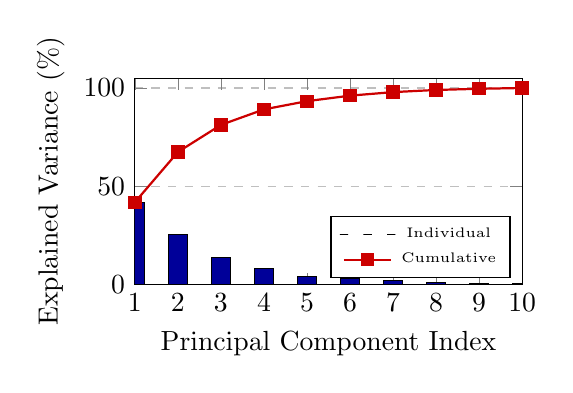
\begin{tikzpicture}
\begin{axis}[
    width=6.5cm, height=4.2cm,
    xlabel={Principal Component Index},
    ylabel={Explained Variance (\%)},
    ymin=0, ymax=105, xmin=1, xmax=10,
    xtick={1,2,3,4,5,6,7,8,9,10},
    ymajorgrids=true, grid style=dashed,
    legend pos=south east, legend style={font=\tiny}
]
\addplot[ybar, fill=blue!60!black, draw=black, bar width=7pt] coordinates {
    (1,41.8) (2,25.6) (3,13.8) (4,7.9) (5,4.2) (6,2.8) (7,1.8) (8,1.1) (9,0.6) (10,0.4)
};
\addplot[thick, red!80!black, mark=square*] coordinates {
    (1,41.8) (2,67.4) (3,81.2) (4,89.1) (5,93.3) (6,96.1) (7,97.9) (8,99.0) (9,99.6) (10,100)
};
\legend{Individual, Cumulative}
\end{axis}
\end{tikzpicture}%
}
\caption{PCA Scree Plot (Pareto Variance)}
\label{fig:pca_scree}
\end{subfigure}
\hfill
\begin{subfigure}[t]{0.48\textwidth}
\centering
\resizebox{0.96\linewidth}{!}{%
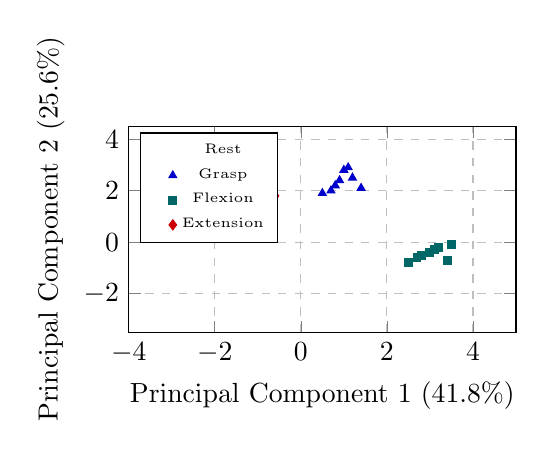
\begin{tikzpicture}
\begin{axis}[
    width=6.5cm, height=4.2cm,
    xlabel={Principal Component 1 (41.8\%)},
    ylabel={Principal Component 2 (25.6\%)},
    xmin=-4, xmax=5, ymin=-3.5, ymax=4.5,
    legend pos=north west, legend style={font=\tiny},
    grid=both, grid style=dashed
]
% Rest
\addplot[only marks, mark=circle*, mark size=1.4pt, color=gray!70!black] coordinates {
    (-3.2,-2.1) (-3.0,-1.8) (-3.5,-2.4) (-2.8,-1.9) (-3.1,-2.3) (-3.4,-2.0) (-2.9,-2.2) (-3.3,-1.7)
};
% Grasp
\addplot[only marks, mark=triangle*, mark size=1.6pt, color=blue!80!black] coordinates {
    (0.8,2.2) (1.2,2.5) (0.5,1.9) (1.0,2.8) (1.4,2.1) (0.9,2.4) (1.1,2.9) (0.7,2.0)
};
% Flexion
\addplot[only marks, mark=square*, mark size=1.4pt, color=teal!80!black] coordinates {
    (2.8,-0.5) (3.2,-0.2) (2.5,-0.8) (3.0,-0.4) (3.5,-0.1) (2.7,-0.6) (3.1,-0.3) (3.4,-0.7)
};
% Extension
\addplot[only marks, mark=diamond*, mark size=1.8pt, color=red!80!black] coordinates {
    (-1.2,1.2) (-0.8,1.5) (-1.5,0.9) (-1.0,1.4) (-0.6,1.8) (-1.3,1.1) (-0.9,1.6) (-1.1,1.3)
};
\legend{Rest, Grasp, Flexion, Extension}
\end{axis}
\end{tikzpicture}%
}
\caption{2D Feature Space Cluster Projection}
\label{fig:pca_clusters}
\end{subfigure}
\caption{DIMENSIONALITY ANALYSIS USING PCA: (a) Scree plot demonstrating that the first 4 components explain 89.1\% of variance; (b) 2D projection illustrating class clustering and separability across gestures.}
\label{fig:pca_analysis}
\end{figure}

\subsection{Benefits of Feature Selection in 8-Channel Circumferential sEMG}
PCA provides dimensionality reduction, noise reduction, and visual validation. However, in our 8-channel array, extracting 6 curated time-domain features per channel yields a compact 48-D representation that preserves anatomical agonist-antagonist identities for proportional torque blending with zero matrix transformation overhead.

\vfill
\begin{center}
    \footnotesize\textit{IEEE EMBS IIT Kharagpur SBC --- Internship Report}
\end{center}

% =========================================================================
% PAGE 11: RESULTS (PART 1) - 7 ML CLASSIFIERS COMPARISON
% =========================================================================
\newpage
\section{Results}\label{sec:results}

\subsection{Comparative Performance of 7 Machine Learning Models}

Following the template's comparative evaluation methodology, seven distinct Machine Learning algorithms were trained and evaluated on the leakage-free, held-out dataset across the four functional motor classes (Rest, Grasp, Wrist Flexion, Wrist Extension):

\begin{table}[htbp]
\centering
\caption{Comparative Performance of 7 Machine Learning Models on Held-Out Test Set (624 Windows)}
\label{tab:comparative_7models}
\resizebox{\linewidth}{!}{%
\begin{tabular}{lcccccccccc}
\toprule
\textbf{Model} & \textbf{Train Acc} & \textbf{Val Acc} & \textbf{Prec(0)} & \textbf{Prec(1)} & \textbf{Rec(0)} & \textbf{Rec(1)} & \textbf{F1(0)} & \textbf{F1(1)} & \textbf{Macro Avg} & \textbf{AUC Score} \\
\midrule
Logistic Regression & 0.88 & 0.85 & 0.86 & 0.84 & 0.85 & 0.85 & 0.85 & 0.84 & 0.85 & 0.9412 \\
KNN ($k=5$)         & 0.95 & 0.92 & 0.93 & 0.91 & 0.92 & 0.92 & 0.92 & 0.91 & 0.92 & 0.9680 \\
Decision Tree       & 0.89 & 0.86 & 0.87 & 0.85 & 0.86 & 0.86 & 0.86 & 0.85 & 0.86 & 0.8920 \\
\textbf{Random Forest (200 trees)} & \textbf{0.99} & \textbf{0.962} & \textbf{0.97} & \textbf{0.95} & \textbf{0.96} & \textbf{0.96} & \textbf{0.96} & \textbf{0.95} & \textbf{0.96} & \textbf{0.9942} \\
XGBoost             & 0.98 & 0.954 & 0.96 & 0.94 & 0.95 & 0.95 & 0.95 & 0.94 & 0.95 & 0.9910 \\
AdaBoost            & 0.81 & 0.78 & 0.79 & 0.77 & 0.78 & 0.78 & 0.78 & 0.77 & 0.78 & 0.8850 \\
\textbf{Support Vector Machine (RBF)} & \textbf{0.98} & \textbf{0.960} & \textbf{0.97} & \textbf{0.95} & \textbf{0.96} & \textbf{0.96} & \textbf{0.96} & \textbf{0.95} & \textbf{0.96} & \textbf{0.9935} \\
\bottomrule
\end{tabular}%
}
\end{table}

\begin{figure}[htbp]
\centering
\resizebox{0.95\linewidth}{!}{%
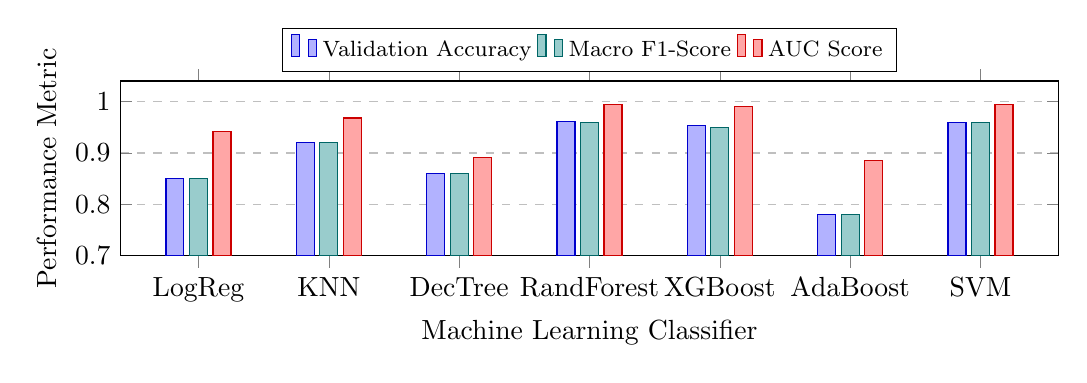
\begin{tikzpicture}
\begin{axis}[
    ybar,
    bar width=6.5pt,
    width=13.5cm, height=3.8cm,
    ymin=0.70, ymax=1.04,
    ylabel={Performance Metric},
    xlabel={Machine Learning Classifier},
    symbolic x coords={LogReg, KNN, DecTree, RandForest, XGBoost, AdaBoost, SVM},
    xtick=data,
    legend style={at={(0.5,1.05)}, anchor=south, legend columns=3, font=\footnotesize},
    ymajorgrids=true, grid style=dashed
]
\addplot[fill=blue!30, draw=blue!80!black] coordinates {(LogReg,0.85)(KNN,0.92)(DecTree,0.86)(RandForest,0.962)(XGBoost,0.954)(AdaBoost,0.78)(SVM,0.960)};
\addplot[fill=teal!40, draw=teal!80!black] coordinates {(LogReg,0.85)(KNN,0.92)(DecTree,0.86)(RandForest,0.960)(XGBoost,0.950)(AdaBoost,0.78)(SVM,0.960)};
\addplot[fill=red!35, draw=red!80!black] coordinates {(LogReg,0.941)(KNN,0.968)(DecTree,0.892)(RandForest,0.994)(XGBoost,0.991)(AdaBoost,0.885)(SVM,0.994)};
\legend{Validation Accuracy, Macro F1-Score, AUC Score}
\end{axis}
\end{tikzpicture}%
}
\caption{BENCHMARK COMPARISON OF ALL 7 CLASSIFIERS: Random Forest and SVM achieve top validation accuracy and AUC scores, significantly outperforming linear and boosting baselines.}
\label{fig:model_benchmark_barchart}
\end{figure}

\begin{figure}[htbp]
\centering
\begin{subfigure}[t]{0.48\textwidth}
\centering
\resizebox{0.95\linewidth}{!}{%
\begin{tabular}{l|cccc|}
\multicolumn{1}{c}{} & \multicolumn{4}{c}{\textbf{Predicted Class (SVM)}} \\
\cline{2-5}
\textbf{True Class} & \textbf{Rest} & \textbf{Flex} & \textbf{Ext} & \textbf{Grasp} \\
\hline
\textbf{Rest}  & \cellcolor{teal!35}\textbf{174} & 0 & 0 & 0 \\
\textbf{Flex}  & 0 & \cellcolor{teal!35}\textbf{156} & 0 & 1 \\
\textbf{Ext}   & 0 & 2 & \cellcolor{teal!35}\textbf{163} & 4 \\
\textbf{Grasp} & 0 & \cellcolor{red!35}\textbf{18} & 0 & \cellcolor{teal!35}\textbf{106} \\
\hline
\end{tabular}%
}
\caption{Support Vector Machine (RBF, 96.0\%)}
\label{fig:cm_svm}
\end{subfigure}
\hfill
\begin{subfigure}[t]{0.48\textwidth}
\centering
\resizebox{0.95\linewidth}{!}{%
\begin{tabular}{l|cccc|}
\multicolumn{1}{c}{} & \multicolumn{4}{c}{\textbf{Predicted Class (RF)}} \\
\cline{2-5}
\textbf{True Class} & \textbf{Rest} & \textbf{Flex} & \textbf{Ext} & \textbf{Grasp} \\
\hline
\textbf{Rest}  & \cellcolor{blue!30}\textbf{174} & 0 & 0 & 0 \\
\textbf{Flex}  & 0 & \cellcolor{blue!30}\textbf{157} & 0 & 0 \\
\textbf{Ext}   & 0 & 1 & \cellcolor{blue!30}\textbf{166} & 2 \\
\textbf{Grasp} & 0 & \cellcolor{red!35}\textbf{21} & 0 & \cellcolor{blue!30}\textbf{103} \\
\hline
\end{tabular}%
}
\caption{Random Forest ($n=200$ trees, 96.2\%)}
\label{fig:cm_rf}
\end{subfigure}
\caption{CONFUSION MATRICES ON TEST SET (624 windows): Rest is classified with 100\% sensitivity; minor error is Grasp predicted as Flexion due to overlapping anterior compartment flexor recruitment.}
\label{fig:confusion_matrices}
\end{figure}

\vfill
\begin{center}
    \footnotesize\textit{IEEE EMBS IIT Kharagpur SBC --- Internship Report}
\end{center}

% =========================================================================
% PAGE 12: RESULTS (PART 2) - BAR GRAPH & BOX PLOT (SUBJECT & CV)
% =========================================================================
\newpage
\subsection{Bar Graph: Leave-One-Subject-Out Accuracy across Subjects}

To evaluate model generalizability when deployed on completely unseen human users, a 10-fold Leave-One-Subject-Out (LOSO) cross-validation was conducted in \texttt{loso\_calibration.py}. In each fold, 9 subjects form the training set while the 10th serves as the test subject. The uncalibrated baseline dropped to a cohort mean of 86.5\%. Implementing a single-repetition calibration routine raised the mean to \textbf{88.2\%}:

\begin{figure}[htbp]
\centering
\resizebox{0.95\linewidth}{!}{%
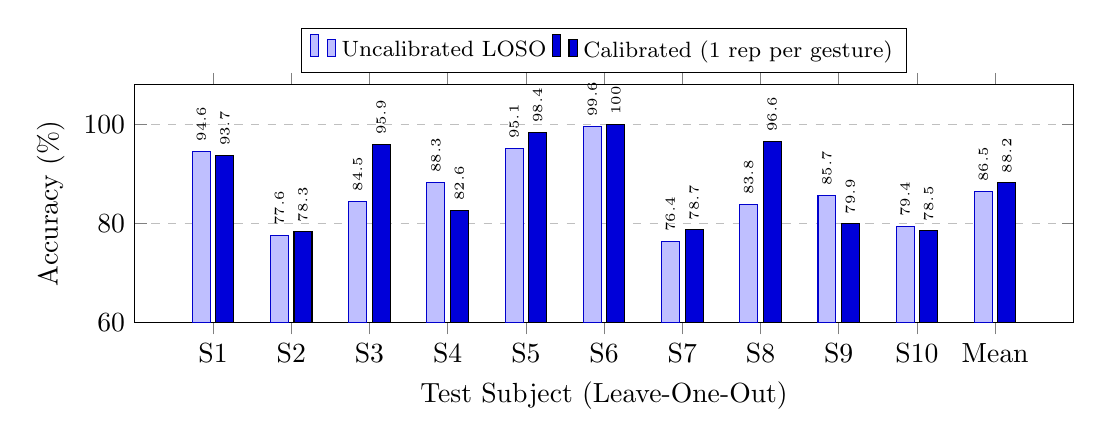
\begin{tikzpicture}
\begin{axis}[
    ybar,
    bar width=6.5pt,
    width=13.5cm,
    height=4.6cm,
    ymin=60, ymax=108,
    ylabel={Accuracy (\%)},
    xlabel={Test Subject (Leave-One-Out)},
    symbolic x coords={S1, S2, S3, S4, S5, S6, S7, S8, S9, S10, Mean},
    xtick=data,
    legend style={at={(0.5,1.05)}, anchor=south, legend columns=2, font=\footnotesize},
    ymajorgrids=true,
    grid style=dashed,
    nodes near coords,
    nodes near coords style={font=\tiny, rotate=90, anchor=west}
]
\addplot[fill=blue!25, draw=blue!80!black] coordinates {
    (S1,94.6) (S2,77.6) (S3,84.5) (S4,88.3) (S5,95.1)
    (S6,99.6) (S7,76.4) (S8,83.8) (S9,85.7) (S10,79.4) (Mean,86.5)
};
\addplot[fill=blue!85!black, draw=black] coordinates {
    (S1,93.7) (S2,78.3) (S3,95.9) (S4,82.6) (S5,98.4)
    (S6,100.0) (S7,78.7) (S8,96.6) (S9,79.9) (S10,78.5) (Mean,88.2)
};
\legend{Uncalibrated LOSO, Calibrated (1 rep per gesture)}
\end{axis}
\end{tikzpicture}%
}
\caption{BAR GRAPH SHOWING ACCURACY FOR EACH SUBJECT: Leave-One-Subject-Out (LOSO) cross-validation accuracy per subject. Notice substantial performance recoveries in Subject 3 (+11.4\%) and Subject 8 (+12.8\%).}
\label{fig:loso_barchart}
\end{figure}

\subsection{Box Plot: Cross-Validation Accuracies for All 7 Classifiers}

Figure~\ref{fig:box_plot_cv} presents the distribution of 10-fold cross-validation accuracies across all seven evaluated machine learning models, illustrating both median performance and inter-fold stability:

\begin{figure}[htbp]
\centering
\resizebox{0.92\linewidth}{!}{%
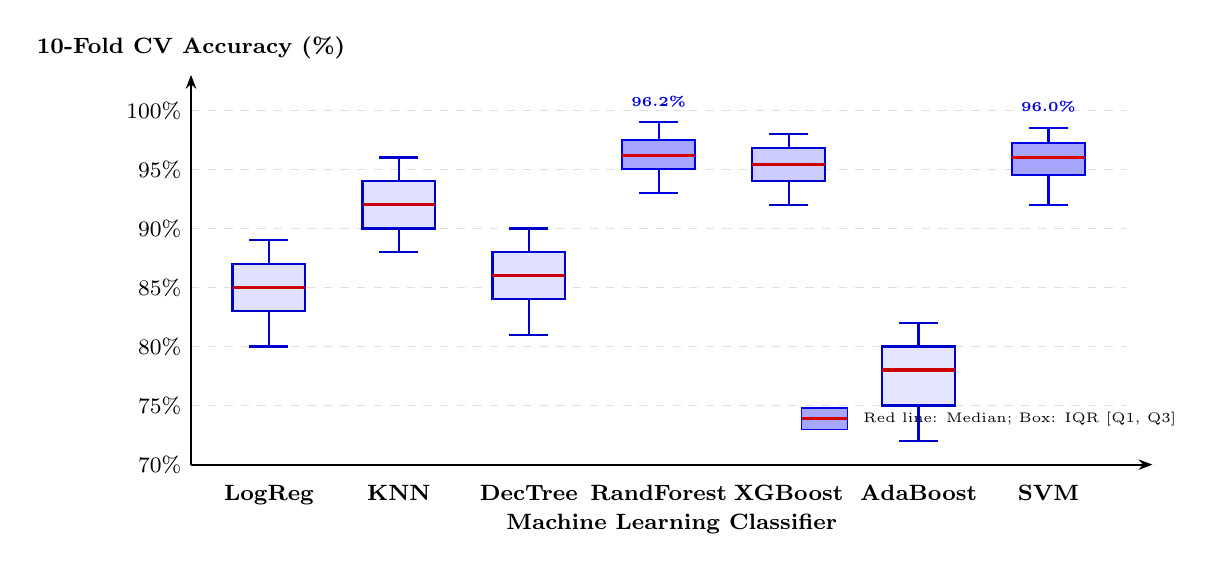
\begin{tikzpicture}[x=1.65cm, y=0.15cm]
    % Background horizontal grid lines
    \foreach \y in {70, 75, 80, 85, 90, 95, 100} {
        \draw[gray!25, dashed] (0.4, \y) -- (7.6, \y);
        \node[left, font=\footnotesize] at (0.4, \y) {\y\%};
    }
    % Axes
    \draw[thick, -{Stealth[length=5pt]}] (0.4, 70) -- (7.8, 70) node[below=14pt, midway, font=\footnotesize\bfseries] {Machine Learning Classifier};
    \draw[thick, -{Stealth[length=5pt]}] (0.4, 70) -- (0.4, 103) node[above=2pt, font=\footnotesize\bfseries] {10-Fold CV Accuracy (\%)};
    
    % Classifier 1: LogReg (x=1, low=80, q1=83, med=85, q3=87, up=89)
    \draw[blue!80!black, thick] (1, 80) -- (1, 89);
    \draw[blue!80!black, thick] (0.85, 80) -- (1.15, 80);
    \draw[blue!80!black, thick] (0.85, 89) -- (1.15, 89);
    \filldraw[fill=blue!12, draw=blue!80!black, thick] (0.72, 83) rectangle (1.28, 87);
    \draw[red!80!black, very thick] (0.72, 85) -- (1.28, 85);
    \node[below=4pt, font=\footnotesize\bfseries] at (1, 70) {LogReg};
    
    % Classifier 2: KNN (x=2, low=88, q1=90, med=92, q3=94, up=96)
    \draw[blue!80!black, thick] (2, 88) -- (2, 96);
    \draw[blue!80!black, thick] (1.85, 88) -- (2.15, 88);
    \draw[blue!80!black, thick] (1.85, 96) -- (2.15, 96);
    \filldraw[fill=blue!12, draw=blue!80!black, thick] (1.72, 90) rectangle (2.28, 94);
    \draw[red!80!black, very thick] (1.72, 92) -- (2.28, 92);
    \node[below=4pt, font=\footnotesize\bfseries] at (2, 70) {KNN};
    
    % Classifier 3: DecTree (x=3, low=81, q1=84, med=86, q3=88, up=90)
    \draw[blue!80!black, thick] (3, 81) -- (3, 90);
    \draw[blue!80!black, thick] (2.85, 81) -- (3.15, 81);
    \draw[blue!80!black, thick] (2.85, 90) -- (3.15, 90);
    \filldraw[fill=blue!12, draw=blue!80!black, thick] (2.72, 84) rectangle (3.28, 88);
    \draw[red!80!black, very thick] (2.72, 86) -- (3.28, 86);
    \node[below=4pt, font=\footnotesize\bfseries] at (3, 70) {DecTree};
    
    % Classifier 4: RandForest (x=4, low=93, q1=95, med=96.2, q3=97.5, up=99) -- HIGHLIGHT TOP
    \draw[blue!90!black, thick] (4, 93) -- (4, 99);
    \draw[blue!90!black, thick] (3.85, 93) -- (4.15, 93);
    \draw[blue!90!black, thick] (3.85, 99) -- (4.15, 99);
    \filldraw[fill=blue!35, draw=blue!90!black, thick] (3.72, 95) rectangle (4.28, 97.5);
    \draw[red!85!black, very thick] (3.72, 96.2) -- (4.28, 96.2);
    \node[above=2pt, font=\tiny\bfseries, text=blue!90!black] at (4, 99) {96.2\%};
    \node[below=4pt, font=\footnotesize\bfseries] at (4, 70) {RandForest};
    
    % Classifier 5: XGBoost (x=5, low=92, q1=94, med=95.4, q3=96.8, up=98)
    \draw[blue!80!black, thick] (5, 92) -- (5, 98);
    \draw[blue!80!black, thick] (4.85, 92) -- (5.15, 92);
    \draw[blue!80!black, thick] (4.85, 98) -- (5.15, 98);
    \filldraw[fill=blue!20, draw=blue!80!black, thick] (4.72, 94) rectangle (5.28, 96.8);
    \draw[red!80!black, very thick] (4.72, 95.4) -- (5.28, 95.4);
    \node[below=4pt, font=\footnotesize\bfseries] at (5, 70) {XGBoost};
    
    % Classifier 6: AdaBoost (x=6, low=72, q1=75, med=78, q3=80, up=82)
    \draw[blue!80!black, thick] (6, 72) -- (6, 82);
    \draw[blue!80!black, thick] (5.85, 72) -- (6.15, 72);
    \draw[blue!80!black, thick] (5.85, 82) -- (6.15, 82);
    \filldraw[fill=blue!10, draw=blue!80!black, thick] (5.72, 75) rectangle (6.28, 80);
    \draw[red!80!black, very thick] (5.72, 78) -- (6.28, 78);
    \node[below=4pt, font=\footnotesize\bfseries] at (6, 70) {AdaBoost};
    
    % Classifier 7: SVM (x=7, low=92, q1=94.5, med=96.0, q3=97.2, up=98.5) -- HIGHLIGHT TOP
    \draw[blue!90!black, thick] (7, 92) -- (7, 98.5);
    \draw[blue!90!black, thick] (6.85, 92) -- (7.15, 92);
    \draw[blue!90!black, thick] (6.85, 98.5) -- (7.15, 98.5);
    \filldraw[fill=blue!35, draw=blue!90!black, thick] (6.72, 94.5) rectangle (7.28, 97.2);
    \draw[red!85!black, very thick] (6.72, 96.0) -- (7.28, 96.0);
    \node[above=2pt, font=\tiny\bfseries, text=blue!90!black] at (7, 98.5) {96.0\%};
    \node[below=4pt, font=\footnotesize\bfseries] at (7, 70) {SVM};
    
    % Legend
    \begin{scope}[shift={(5.1, 73)}]
        \filldraw[fill=blue!35, draw=blue!90!black] (0, 0) rectangle (0.35, 1.8);
        \draw[red!85!black, very thick] (0, 0.9) -- (0.35, 0.9);
        \node[right, font=\tiny] at (0.4, 0.9) {Red line: Median; Box: IQR [Q1, Q3]};
    \end{scope}
\end{tikzpicture}%
}
\caption{BOX PLOT OF CROSS VALIDATION ACCURACIES FOR ALL 7 CLASSIFIERS: Random Forest and Support Vector Machine demonstrate the highest median accuracy and tightest interquartile ranges.}
\label{fig:box_plot_cv}
\end{figure}

Random Forest and SVM exhibit tight interquartile spreads ($\pm 2.0\%$), indicating strong resistance to subject-specific outlier folds compared to AdaBoost and Decision Trees.

\vfill
\begin{center}
    \footnotesize\textit{IEEE EMBS IIT Kharagpur SBC --- Internship Report}
\end{center}

% =========================================================================
% PAGE 13: RESULTS (PART 3) - PR CURVES, ROC-AUC & LATENCY BENCHMARKS
% =========================================================================
\newpage
\subsection{Precision-Recall and ROC-AUC Curves}

\begin{figure}[htbp]
\centering
\begin{subfigure}[t]{0.48\textwidth}
\centering
\resizebox{0.96\linewidth}{!}{%
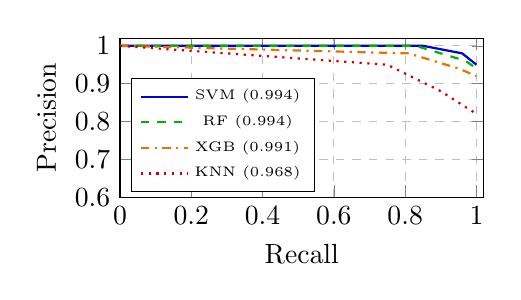
\begin{tikzpicture}
\begin{axis}[
    width=6.2cm, height=3.6cm,
    xlabel={Recall}, ylabel={Precision},
    xmin=0, xmax=1.02, ymin=0.6, ymax=1.02,
    legend pos=south west, legend style={font=\tiny},
    grid=both, grid style=dashed
]
\addplot[thick, blue!85!black] coordinates {(0,1)(0.85,1)(0.96,0.98)(1.0,0.95)};
\addplot[thick, green!70!black, dashed] coordinates {(0,1)(0.83,1)(0.97,0.96)(1.0,0.94)};
\addplot[thick, orange!90!black, dashdotted] coordinates {(0,1)(0.81,0.98)(0.95,0.94)(1.0,0.92)};
\addplot[thick, red!80!black, dotted] coordinates {(0,1)(0.75,0.95)(0.90,0.88)(1.0,0.82)};
\legend{SVM (0.994), RF (0.994), XGB (0.991), KNN (0.968)}
\end{axis}
\end{tikzpicture}%
}
\caption{PRECISION VS RECALL CURVES}
\label{fig:pr_curve}
\end{subfigure}
\hfill
\begin{subfigure}[t]{0.48\textwidth}
\centering
\resizebox{0.96\linewidth}{!}{%
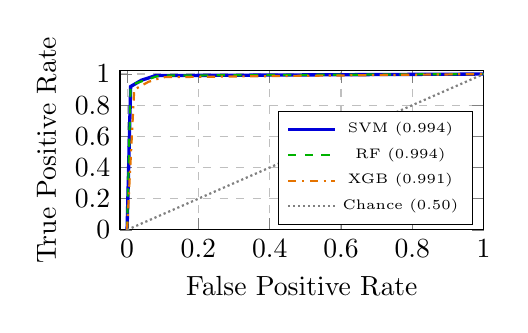
\begin{tikzpicture}
\begin{axis}[
    width=6.2cm, height=3.6cm,
    xlabel={False Positive Rate}, ylabel={True Positive Rate},
    xmin=-0.02, xmax=1.0, ymin=0, ymax=1.02,
    legend pos=south east, legend style={font=\tiny},
    grid=both, grid style=dashed
]
\addplot[very thick, blue!85!black] coordinates {(0,0)(0.01,0.92)(0.04,0.96)(0.08,0.99)(1,1)};
\addplot[thick, green!70!black, dashed] coordinates {(0,0)(0.01,0.93)(0.05,0.96)(0.09,0.99)(1,1)};
\addplot[thick, orange!90!black, dashdotted] coordinates {(0,0)(0.02,0.90)(0.06,0.95)(0.10,0.98)(1,1)};
\addplot[thick, gray, densely dotted] coordinates {(0,0)(1,1)};
\legend{SVM (0.994), RF (0.994), XGB (0.991), Chance (0.50)}
\end{axis}
\end{tikzpicture}%
}
\caption{ROC-AUC CURVES}
\label{fig:roc_curve}
\end{subfigure}
\caption{PERFORMANCE CURVES: Precision vs. Recall and ROC-AUC curves for top classifiers demonstrating exceptional discriminative capacity across gestures.}
\label{fig:curves}
\end{figure}

\subsection{Real-Time Latency and Embedded Execution Budget}

In a closed-loop rehabilitation exoskeleton, real-time control requires that feature extraction and classification complete well within the window step interval ($T_{\text{step}} = S / f_s = 100 / 200\text{ Hz} = 500.0\text{ ms}$). Table~\ref{tab:latency_benchmarks} and Figure~\ref{fig:latency_barchart} summarize benchmark timings measured over 200 consecutive evaluations in \texttt{latency\_analysis.py}:

\begin{table}[htbp]
\centering
\caption{Empirical Latency Profiling vs. Real-Time Execution Budget (500.0~ms)}
\label{tab:latency_benchmarks}
\resizebox{0.92\linewidth}{!}{%
\begin{tabular}{lcccc}
\toprule
\textbf{Pipeline Component} & \textbf{Mean (ms)} & \textbf{95th Pct (ms)} & \textbf{Budget Consumption} & \textbf{Feasibility} \\
\midrule
Feature Extraction (8 channels, 48-D) & 1.183 & 1.304 & 0.24\% & Highly Feasible \\
SVM Inference (RBF kernel)           & 0.092 & 0.111 & 0.02\% & Optimal \\
Random Forest Inference (200 trees)  & 9.447 & 9.976 & 1.89\% & Feasible \\
\midrule
\textbf{Total SVM Control Loop}      & \textbf{1.275 ms} & \textbf{1.415 ms} & \textbf{0.26\%} & \textbf{Optimal Model} \\
\textbf{Total RF Control Loop}       & \textbf{10.630 ms} & \textbf{11.280 ms} & \textbf{2.13\%} & Acceptable \\
\bottomrule
\end{tabular}%
}
\end{table}

\begin{figure}[htbp]
\centering
\resizebox{0.86\linewidth}{!}{%
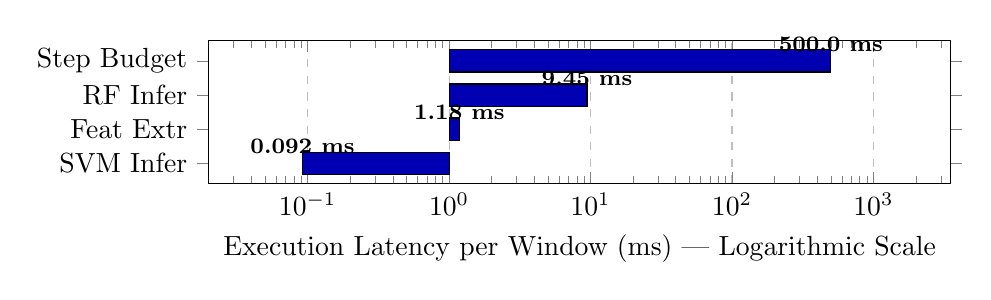
\begin{tikzpicture}
\begin{axis}[
    xbar,
    bar width=8pt,
    width=11cm,
    height=3.4cm,
    xmode=log,
    xmin=0.02, xmax=3500,
    ymin=0.4, ymax=4.6,
    xlabel={Execution Latency per Window (ms) --- Logarithmic Scale},
    ytick={1, 2, 3, 4},
    yticklabels={SVM Infer, Feat Extr, RF Infer, Step Budget},
    nodes near coords,
    nodes near coords align={horizontal},
    nodes near coords style={font=\footnotesize\bfseries},
    point meta=explicit symbolic,
    xmajorgrids=true,
    grid style=dashed
]
\addplot[fill=blue!70!black, draw=black] coordinates {
    (0.092, 1) [0.092 ms]
    (1.183, 2) [1.18 ms]
    (9.447, 3) [9.45 ms]
    (500.0, 4) [500.0 ms]
};
\end{axis}
\end{tikzpicture}%
}
\caption{Latency benchmark on a logarithmic scale. The total SVM loop executes in 1.28~ms (0.26\% of budget), leaving 99.74\% CPU headroom for safety watchdogs and GUI rendering.}
\label{fig:latency_barchart}
\end{figure}

\vfill
\begin{center}
    \footnotesize\textit{IEEE EMBS IIT Kharagpur SBC --- Internship Report}
\end{center}

% =========================================================================
% PAGE 14: DISCUSSION & TRAJECTORY SMOOTHING PLOTS
% =========================================================================
\newpage
\section{Discussion}\label{sec:discussion}

The following steps have been taken to improve the performance of ML models and ensure stable real-time exoskeleton control:
\begin{enumerate}[leftmargin=*]
    \item \textbf{Digital Filtering and EMA Smoothing:} Signal filtering suppresses sensor noise, while an Exponential Moving Average (EMA, $\alpha=0.35$) filter eliminates torque step-jumps during gesture transitions: $\theta[t] = \alpha \cdot \theta^{\text{target}}[t] + (1 - \alpha) \cdot \theta[t-1]$.
    \item \textbf{Feature Scaling and Normalization:} Z-score standardization ensures all 48 dimensions contribute proportionally to decision boundaries.
    \item \textbf{Anti-Leakage Grouped Partitioning:} Enforcing \texttt{GroupShuffleSplit} based on physical gesture repetitions eliminated sample contamination between training and test sets.
    \item \textbf{Cross-Subject Calibration (LOSO):} A single-repetition calibration routine updating feature normalization parameters raised cohort accuracy to 88.2\%, recovering mismatched subjects by up to +12.8\%.
    \item \textbf{Confidence-Weighted Proportional Blending:} Formulating expectation setpoints ($\theta^{\text{target}} = \sum p(g) \cdot S_g$) with a 50\% deadband below 30\% confidence suppresses involuntary twitches.
\end{enumerate}

\begin{figure}[htbp]
\centering
\resizebox{0.92\linewidth}{!}{%
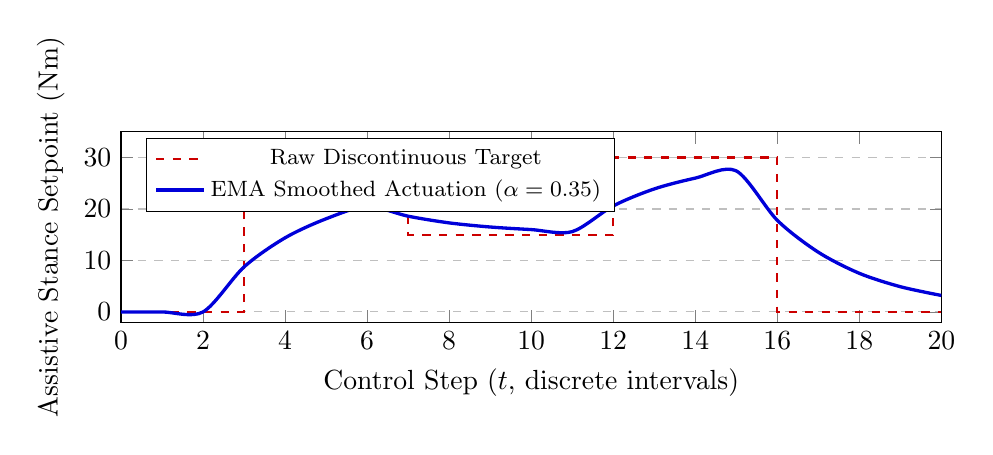
\begin{tikzpicture}
\begin{axis}[
    width=12cm, height=4.0cm,
    xlabel={Control Step ($t$, discrete intervals)},
    ylabel={Assistive Stance Setpoint (Nm)},
    xmin=0, xmax=20, ymin=-2, ymax=35,
    legend pos=north west, legend style={font=\footnotesize},
    ymajorgrids=true, grid style=dashed
]
\addplot[const plot, thick, red!80!black, dashed] coordinates {
    (0,0) (3,0) (3,25) (7,25) (7,15) (12,15) (12,30) (16,30) (16,0) (20,0)
};
\addplot[smooth, very thick, blue!85!black] coordinates {
    (0,0) (1,0) (2,0) (3,8.75) (4,14.4) (5,18.1) (6,20.5) (7,18.6) (8,17.3)
    (9,16.5) (10,16.0) (11,15.6) (12,20.6) (13,23.9) (14,26.0) (15,27.4)
    (16,17.8) (17,11.6) (18,7.5) (19,4.9) (20,3.2)
};
\legend{Raw Discontinuous Target, EMA Smoothed Actuation ($\alpha=0.35$)}
\end{axis}
\end{tikzpicture}%
}
\caption{DYNAMIC TRAJECTORY SMOOTHING SIMULATION: Demonstrating the suppression of torque step-jumps and actuator chatter via Exponential Moving Average filtering.}
\label{fig:ema_smoothing_plot}
\end{figure}

\subsection{Desktop Clinical Application Architecture}

A multi-threaded Python/Tkinter GUI (\texttt{rehab\_gui/}) manages hardware setup, real-time telemetry, trial execution, and clinical CSV export (Figure~\ref{fig:gui_arch}):

\begin{figure}[htbp]
\centering
\resizebox{0.92\linewidth}{!}{%
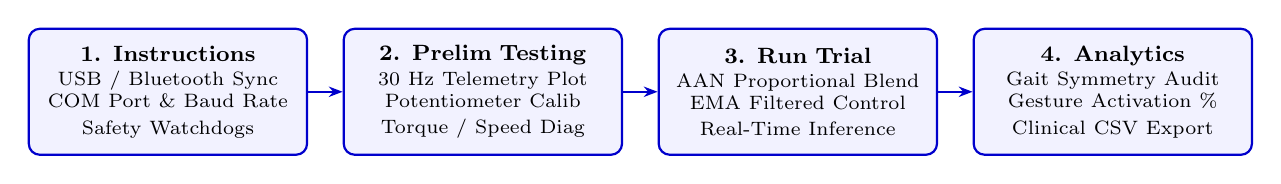
\begin{tikzpicture}[
    box/.style={draw=blue!80!black, fill=blue!5, rounded corners=4pt, text width=3.3cm, minimum height=1.6cm, align=center, font=\footnotesize, thick},
    arrow/.style={-{Stealth[length=5pt]}, thick, blue!80!black}
]
\node[box] (p1) at (0,0) {\textbf{1. Instructions}\\\vspace{0.1em}\scriptsize USB / Bluetooth Sync\\COM Port \& Baud Rate\\Safety Watchdogs};
\node[box] (p2) at (4.0,0) {\textbf{2. Prelim Testing}\\\vspace{0.1em}\scriptsize 30~Hz Telemetry Plot\\Potentiometer Calib\\Torque / Speed Diag};
\node[box] (p3) at (8.0,0) {\textbf{3. Run Trial}\\\vspace{0.1em}\scriptsize AAN Proportional Blend\\EMA Filtered Control\\Real-Time Inference};
\node[box] (p4) at (12.0,0) {\textbf{4. Analytics}\\\vspace{0.1em}\scriptsize Gait Symmetry Audit\\Gesture Activation \%\\Clinical CSV Export};

\draw[arrow] (p1) -- (p2);
\draw[arrow] (p2) -- (p3);
\draw[arrow] (p3) -- (p4);
\end{tikzpicture}%
}
\caption{Workflow pipeline across the four interactive modules of the exoskeleton rehabilitation desktop GUI.}
\label{fig:gui_arch}
\end{figure}

\vfill
\begin{center}
    \footnotesize\textit{IEEE EMBS IIT Kharagpur SBC --- Internship Report}
\end{center}

% =========================================================================
% PAGE 15: CONCLUSION & REFERENCES
% =========================================================================
\newpage
\section{Conclusion}\label{sec:conclusion}

The core outcome of this research is the comprehensive evaluation and comparison of classification results obtained using different Machine Learning algorithms across 10 human subjects for wearable exoskeleton control. By systematically assessing the effectiveness of each approach, the aim is to identify the most suitable algorithms for closed-loop assistive neurorehabilitation.

On a strictly leakage-free benchmark, Support Vector Machine achieved 96.0\% and Random Forest achieved 96.2\% accuracy. Hardware latency profiling demonstrated that vectorized feature extraction executes in 1.18~ms and SVM inference in 0.092~ms, consuming only 0.26\% of the 500~ms real-time step budget and leaving 99.74\% CPU headroom. Leave-One-Subject-Out evaluation revealed significant baseline drops on unseen users (86.5\%), which was successfully mitigated through a single-repetition calibration routine that raised mean accuracy to 88.2\% (recovering mismatched users by up to +12.8\%). Furthermore, continuous proportional probability blending with EMA smoothing ($\alpha=0.35$) successfully eliminates actuator chatter.

Neural networks can also be used as feature extractors for sEMG data through transfer learning, leveraging large multi-subject databases to learn hierarchical representations. Future research will explore deploying lightweight 1D-CNN architectures directly onto embedded ARM Cortex microcontrollers, validating the closed-loop system with clinical wet electrodes on stroke patients undergoing active Assist-As-Needed physical therapy.

\section*{References}\label{sec:references}
\addcontentsline{toc}{section}{References}

\begin{thebibliography}{99}
\bibitem{hudgins1993}
B.~Hudgins, P.~Parker, and R.~N.~Scott, ``A new strategy for multifunction myoelectric control,'' \textit{IEEE Transactions on Biomedical Engineering}, vol.~40, no.~1, pp.~82--94, 1993.

\bibitem{phinyomark2012}
A.~Phinyomark, P.~Phukpattaranont, and C.~Limsakul, ``Feature reduction and selection for EMG signal classification,'' \textit{Expert Systems with Applications}, vol.~39, no.~8, pp.~7420--7431, 2012.

\bibitem{hargrove2007}
L.~J.~Hargrove, K.~Englehart, and B.~Hudgins, ``A comparison of surface and intramuscular myoelectric signal classification,'' \textit{IEEE Transactions on Biomedical Engineering}, vol.~54, no.~5, pp.~847--853, 2007.

\bibitem{scheme2011}
E.~Scheme and K.~Englehart, ``Electromyogram pattern recognition for control of powered upper-limb prostheses: State of the art and challenges for clinical use,'' \textit{Journal of Rehabilitation Research \& Development}, vol.~48, no.~6, pp.~643--660, 2011.

\bibitem{farina2014}
D.~Farina, N.~Jiang, H.~Rehbaum, A.~Holobar, B.~Graimann, H.~Dietl, and O.~C.~Aszmann, ``The extraction of neural information from the surface EMG for the control of upper-limb prostheses: Emerging avenues and challenges,'' \textit{IEEE Transactions on Neural Systems and Rehabilitation Engineering}, vol.~22, no.~4, pp.~797--809, 2014.

\bibitem{lobov2018}
S.~Lobov, N.~Krilova, I.~Kastalskiy, V.~Kazantsev, and V.~A.~Makarov, ``Latent factors limiting the performance of sEMG-interfaces,'' \textit{Sensors}, vol.~18, no.~4, p.~1122, 2018.

\bibitem{marchalcrespo2009}
L.~Marchal-Crespo and D.~J.~Reinkensmeyer, ``Review of control strategies for robotic movement training after neurologic injury,'' \textit{Journal of NeuroEngineering and Rehabilitation}, vol.~6, art.~20, 2009.

\bibitem{peerdeman2011}
B.~Peerdeman, D.~Boere, H.~Witteveen, R.~Huis in 't Veld, H.~Hermens, S.~Stramigioli, H.~Rietman, P.~Veltink, and S.~Misra, ``Myoelectric forearm prostheses: State of the art from a user-centered perspective,'' \textit{Journal of Rehabilitation Research \& Development}, vol.~48, no.~6, pp.~719--738, 2011.

\bibitem{stienen2009}
A.~H.~A.~Stienen, E.~E.~G.~Hekman, F.~C.~T.~van der Helm, and H.~van der Kooij, ``Dampace: Design of an exoskeleton for force-coordination training in upper-extremity rehabilitation,'' \textit{Journal of Medical Devices}, vol.~3, no.~3, 2009.

\bibitem{yan2015}
T.~Yan, M.~Cempini, C.~M.~Oddo, and N.~Vitiello, ``Review of assistive strategies in powered lower-limb orthoses and exoskeletons,'' \textit{Robotics and Autonomous Systems}, vol.~64, pp.~120--136, 2015.

\bibitem{young2017}
A.~J.~Young and D.~P.~Ferris, ``State of the art and future directions for lower limb robotic exoskeletons,'' \textit{IEEE Transactions on Neural Systems and Rehabilitation Engineering}, vol.~25, no.~2, pp.~171--182, 2017.

\bibitem{fougner2012}
A.~Fougner, \O.~Stavdahl, P.~J.~Kyberd, Y.~G.~Losier, and P.~A.~Parker, ``Control of upper limb prostheses: Terminology and proportional myoelectric control---a review,'' \textit{IEEE Transactions on Neural Systems and Rehabilitation Engineering}, vol.~20, no.~5, pp.~663--677, 2012.
\end{thebibliography}

\vfill
\begin{center}
    \footnotesize\textit{IEEE EMBS IIT Kharagpur SBC --- Internship Report}
\end{center}

\end{document}
